\documentclass[12pt, letterpaper]{article}
\usepackage[titletoc,title]{appendix}
\usepackage{color}
\usepackage{booktabs}
\usepackage{caption}
\newcommand\fnote[1]{\captionsetup{font=small}\caption*{#1}}
\usepackage{float}
\usepackage[scaled=.7]{beramono}
\usepackage[usenames,dvipsnames,svgnames,table]{xcolor}
\definecolor{dark-red}{rgb}{0.75,0.10,0.10} 
\usepackage[margin=1in]{geometry}
\usepackage[linkcolor=blue,
            colorlinks=true,
            urlcolor=blue,
            pdfstartview={XYZ null null 1.00},
            pdfpagemode=UseNone,
            citecolor={blue},
            pdftitle={Not News}]{hyperref}

\usepackage{multibib}
\usepackage{geometry} % see geometry.pdf on how to lay out the page. There's lots.
\geometry{letterpaper}               % This is 8.5x11 paper. Options are a4paper or a5paper or other... 
\usepackage{graphicx}                % Handles inclusion of major graphics formats and allows use of 
\usepackage{amsfonts,amssymb,amsbsy}
\usepackage{amsxtra}
\usepackage{natbib}
\usepackage{longtable}
\usepackage{array}
\usepackage{multirow}
\usepackage{wrapfig}
\usepackage{colortbl}
\usepackage{pdflscape}
\usepackage{tabu}
\usepackage{threeparttable}
\usepackage{threeparttablex}
\usepackage[normalem]{ulem}
\usepackage{makecell}
\usepackage{verbatim}
\setcitestyle{round,semicolon,aysep={},yysep={;}}
\usepackage{setspace}             % Permits line spacing control. Options are \doublespacing, \onehalfspace
\usepackage{sectsty}             % Permits control of section header styles
\usepackage{lscape}
\usepackage{fancyhdr}             % Permits header customization. See header section below.
\usepackage{url}                 % Correctly formats URLs with the \url{} tag
\usepackage{fullpage}             %1-inch margins
\usepackage{multirow}
\usepackage{rotating}
\setlength{\parindent}{3em}
\usepackage{subcaption}
\usepackage[T1]{fontenc}
\usepackage{libertine}
\usepackage{inconsolata}
%\usepackage{babel}
\title{\Large{Birthday Voter}\footnote{Scripts behind the analysis can be downloaded at: \url{https://github.com/soodoku/birthday_voter}.}}
\author{Jake Leland\thanks{Jake can be reached at \href{mailto:jake.leland@utexas.edu}{\footnotesize{\texttt{jakebleland@gmail.com}}}}
\and Gaurav Sood\thanks{Gaurav can be reached at \href{mailto:gsood07@gmail.com}{\footnotesize{\texttt{gsood07@gmail.com}}}}}

\date{\vspace{.5cm}\normalsize{\today}}

\begin{document}
\maketitle

\begin{comment}

setwd(paste0(githubdir, "birthday_voter/ms"))
tools::texi2dvi("birthday_voter.tex", pdf = TRUE, clean = TRUE) 
setwd(basedir)

\end{comment}

\begin{abstract}

\end{abstract}

\clearpage
\doublespacing
We leverage data on millions of people using Florida state voter registration files to estimate whether people turn out more often if their birthday falls on the voting day. We conjecture that people see voting as a duty, and like doing dutiful things on their birthdays. To the extent that is true, it gives us evidence for voting as a duty. In addition, voting more frequently on birthdays may also be driven by people taking the day off on their birthdays and using the time to vote. To the extent that is the reason behind it, making election day an official holiday would increase turnout.

\section{Data and Measurement}
The dataset was extracted as of February 2017 and includes 10 years of elections from 2006 through 2016. There are two files.

\begin{itemize}
	\item \textbf{Official voter registration information}: Data is extracted from the Florida Voter Registration System and includes information on voters who are officially registered or pre-registered as of the end of the prior month. All information is included except limited in those cases in which a voter requested exemption from public disclosure per Section 119.071, Fla. Stat.  (Section 98.0981(1)(b), Fla. Stat.).

	\item \textbf{Unofficial voting history information} Data is extracted from independently submitted reports from the 67 county supervisors of elections capturing voting history at a fixed point in time. 
\end{itemize}

\subsection{Data Validation}

We apply a set of filters to ensure that only persons at least 18 years old and registered to vote on election day are included in the analysis. We also perform a set of validation checks to confirm the soundness and accuracy of the dataset.

\begin{itemize}

	\item \textbf{Fake Birthdays}: we search for potential fake birthdays by identifying a month and day of year with a high number of occurrences (e.g. if an unusually high number of voters brithdays fall on a specific day).

	\item \textbf{Voter turnout grouped by age}: we expect to see turnout initially go down until mid 20s, then increase steadily until about 70-80 years before declining.

	\item \textbf{Voter turnout during midterms vs. presidential elections}: we expect to see higher turnout for presidential elections than midterms.

	\item \textbf{Voter turnout during general vs. primary elections}: we expect to see higher turnout for general elections than primaries.

\end{itemize}

The dataset passed the validation checks. For the purposes of this analysis, we also limit the data to primary and general elections receiving at least 100 thousand votes. 

\section{Results}
We get the cartesian product of the voter registration file and the voting history file, such that primary key of the dataset is $voter_id | election_type | election_date$. We then group by the number of days between the person’s birthday and the election date, and calculate the mean change in voter turnout from the previous day. The analysis shows a substantial increase in turnout if election day falls on the voter’s birthday, as displayed in figure 1.

\begin{figure}[H]
\centering
 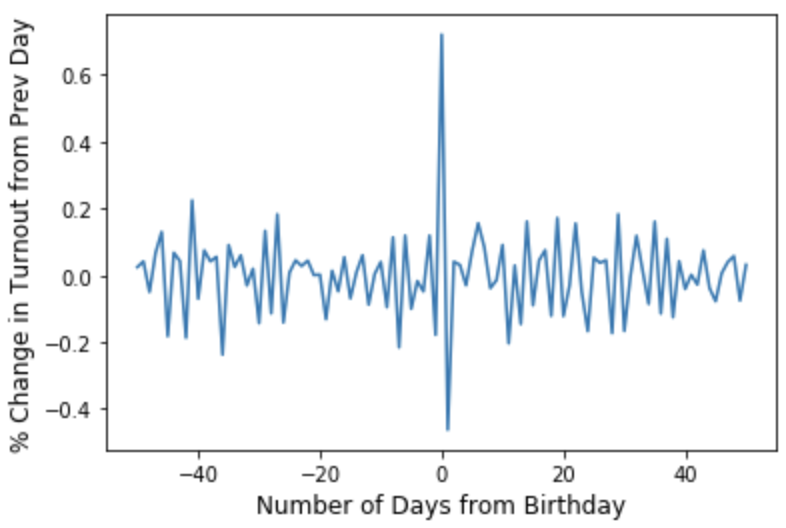
\includegraphics[scale=.7]{../figs/fig1.png}
 \caption{Birthday Voter}
 \label{fig:birthday}
\end{figure}

Tables 1, 2 and 3 show the mean absolute change in turnout for when the election date falls $+/- 50 days,+/-  30 days, and +/- 7$ days from the voter's birthday compared to when the election falls on the voter's birthday. In all three cases, the change in turnout from the previous day is more than two times greater when election date falls on the voter’s birthday.

\section{Conclusion}
Further research may be warranted to determine the causal relationship between a person's birthday and voting, which may be a result of a sense of duty, having more leisure time, or simply making it easier to remember. Whatever the case may be, our analysis shows that a person is in fact more likely to vote when election day falls on their birthday. 

\clearpage
\bibliographystyle{apsr}
\bibliography{birthday_voter}  

\clearpage
\appendix
\renewcommand{\thesection}{SI \arabic{section}}
\renewcommand\thetable{\thesection.\arabic{table}}  
\renewcommand\thefigure{\thesection.\arabic{figure}}
\counterwithin{figure}{section}

\section{Supporting Information}

\end{document}